\chapter{Results}
\label{cha:results}

%This chapter presents the results. Note that the results are presented
%factually, striving for objectivity as far as possible.  The results
%shall not be analyzed, discussed or evaluated.  This is left for the
%discussion chapter.

%In case the method chapter has been divided into subheadings such as
%pre-study, implementation and evaluation, the result chapter should
%have the same sub-headings. This gives a clear structure and makes the
%chapter easier to write.

%In case results are presented from a process (e.g. an implementation
%process), the main decisions made during the process must be clearly
%presented and justified. Normally, alternative attempts, etc, have
%already been described in the theory chapter, making it possible to
%refer to it as part of the justification.

In this chapter the results are described.
First, the outcome from the exploratory study is presented, followed by the different experiments.
The first experiment, filtering out invalid reports, presents the evaluation of the topic model used to filter out the reports, as well as the specific topics and how they were used in the process.
In the second one, the methods considered and the decisions behind which ones that were appropriate are presented.
Finally, the last section goes through the result of evaluating the different active learning techniques.

\section{Exploratory Study}

The goal with the exploratory study was to acquire a better understanding of the data, how it was structured and what kind of information might be extracted from it.
%[FIGURE FROM METHOD] displayed popular terms from a subset of the topics obtained from the topic model.
Certain fields such as the cancelled field did not seem to be very reliable. 
Reports that clearly explained a situation where the patient had been transferred to another hospital, or for another reason not having performed an examination, still described a situation where the cancelled field was set to ``false''.
After further manual analysis it was clear that the vast amount of invalid reports were contained within a few topics, something that is used in the first research question.
The evaluation of more concrete relationships were done within the context of that experiment, and is presented in Section~\ref{sec:exp1-result}.

The word2vec model produced results that allowed for synonyms to be detected.
By doing this, 420 pairs were discovered.
The vast majority of these were names and words that are used in similar contexts, which includes opposites like ``left'' and ``right''.
Some of the medical terms was hard to interpret, and were therefore not considered to be synonyms.
Disregarding these, the synonyms and misspellings that were decided for use in the final system can be seen in Table~\ref{tab:synonyms}.
The original value was replaced with the new one in the final system.

\begin{table}
    \centering
    \begin{tabular}{|ccc|}
        \hline
        \textbf{Original} & \textbf{Replacement} & \textbf{Type} \\
        \hline
        ordinärt & normalt & synonyms \\
        ej & inte & synonyms \\
        avbeställd & avbokad & synonyms \\
        avebställd & avbokad & misspelling + synonym \\
        belsutat & beslutat & misspelling \\
        måttliga & lätta & synonyms \\
        pat & patient & short \\
        pt & patient & short \\
        pateint & patient & misspelling \\
        akuten & akutmottagningen & misspelling \\
        us & undersökning & short \\
        \hline
    \end{tabular}
    \caption{The synonyms, misspellings and shorts found in the data that the author could with assert with confidence.}
    \label{tab:synonyms}
\end{table}

In order to identify names from this word2vec model, the word vectors were plotted using the an interactive plot that allowed for exploration of the data.
Since names are commonly used in similar contexts, they would have similar attributes in the word embedding model.
Figure~\ref{fig:word2vec-names-overview} shows how this was done.
Given that the names got similar coordinates in the plot, identifying the section with names allowed for identification of a lot of the names used in the reports.

\begin{figure}
    \begin{subfigure}[b]{\textwidth}
        \centering
        \fbox{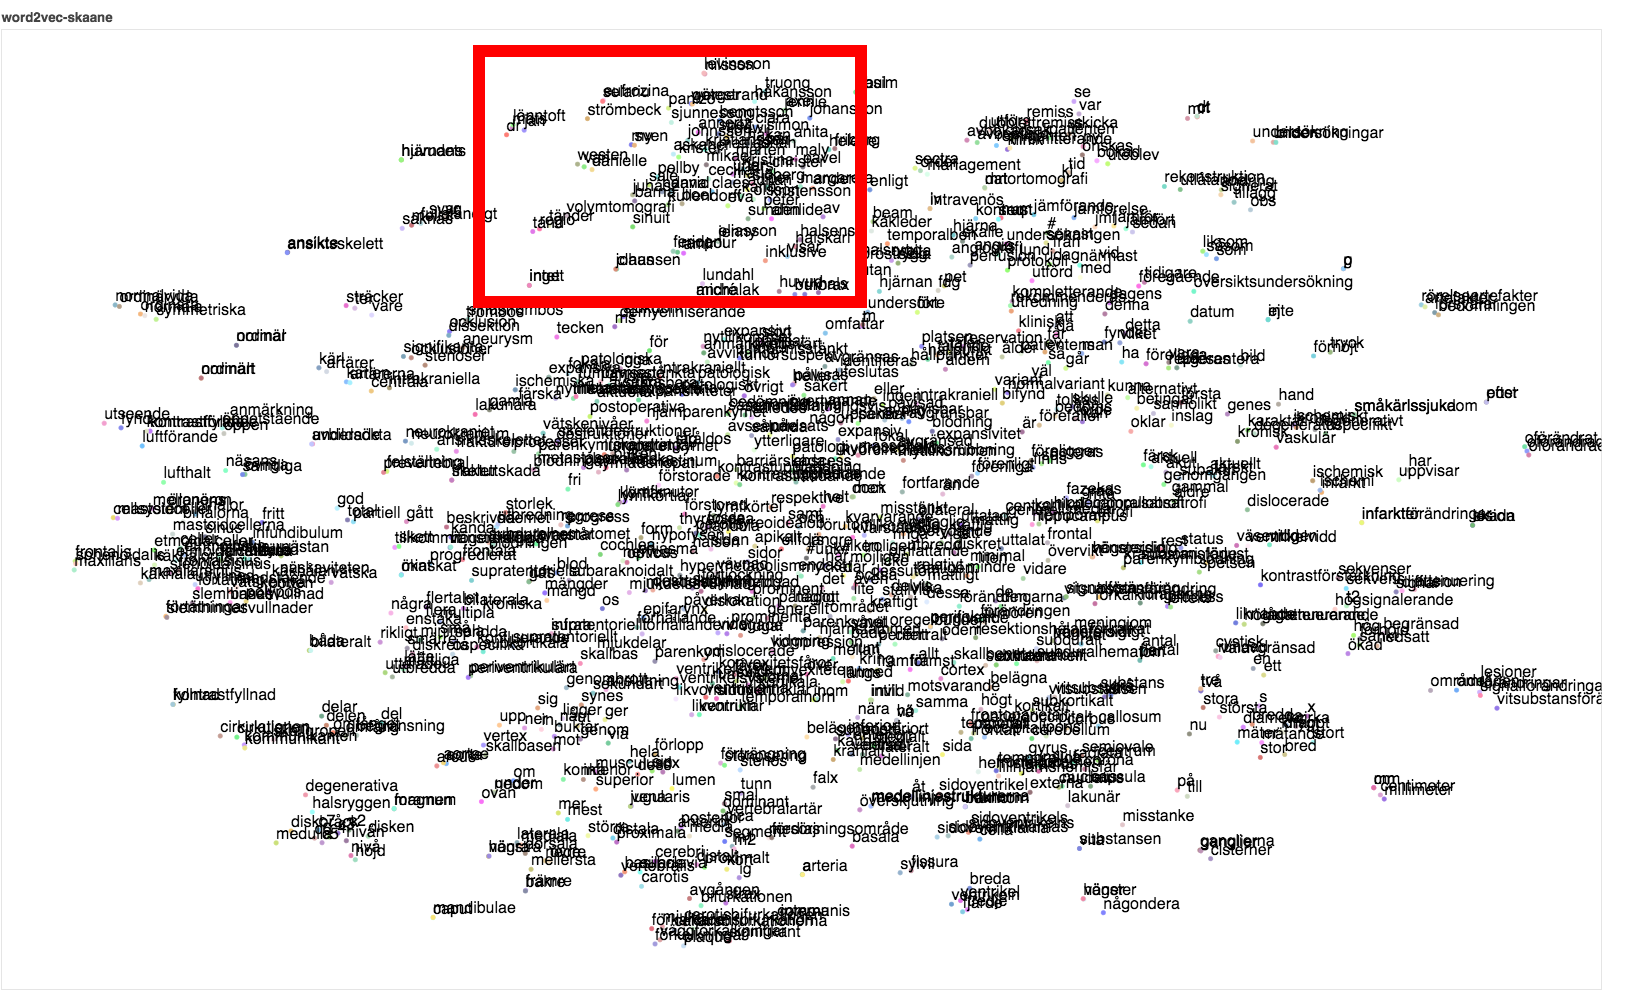
\includegraphics[scale=0.25]{figures/word2vec-overview.png}}
        \caption{A 2D plot of the full word2vec model.}
    \end{subfigure}
    \quad
    \begin{subfigure}[b]{\textwidth}
        \centering
        \fbox{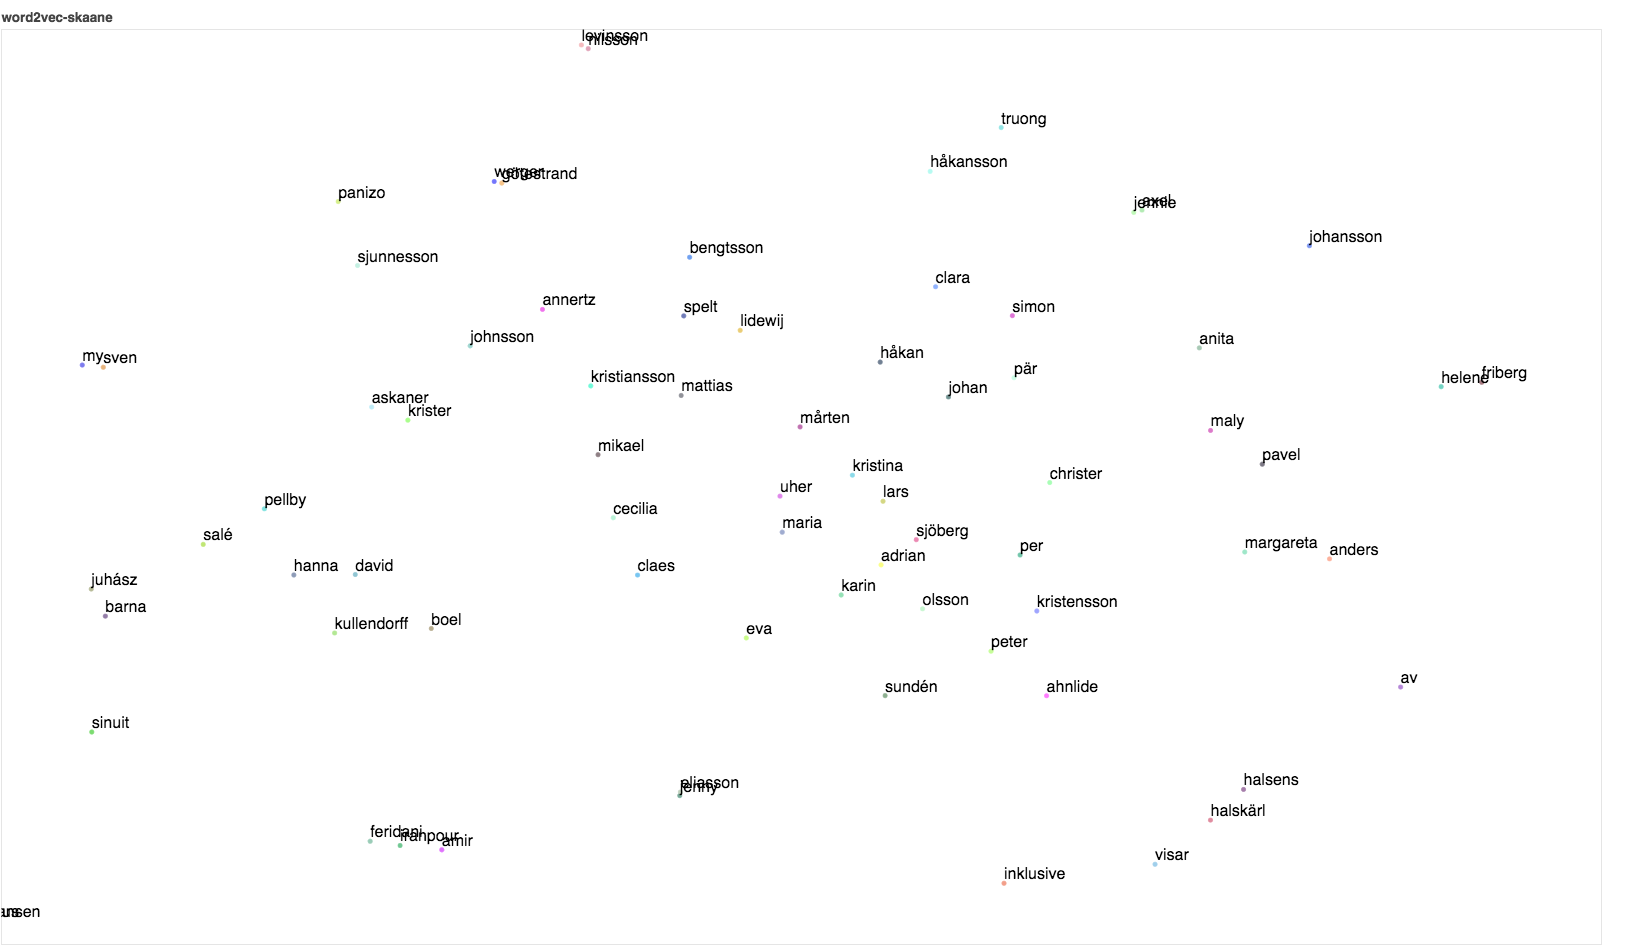
\includegraphics[scale=0.25]{figures/word2vec-names.png}}
        \caption{A 2D plot of the subset of the word2vec model covering the names.}
    \end{subfigure}
    \caption{Two figures illustrating how the names were discovered in the word2vec plot. The (b) plot represents the red square in (a).}
    \label{fig:word2vec-names-overview}
\end{figure}

\section{Filter Out Invalid Clinical Reports Using Topic Models and Clustering}\label{sec:exp1-result}

The LDA models were evaluated by calculating the perplexity on the held-out set as described in Section~\ref{sec:exp1-method}.
Perplexity for the evaluated models can be seen in Figure~\ref{fig:lda-perplexity}, where a low score is better.
Based on this, the selected model was the LDA model with 75 topics.

\begin{figure}[h!]
    \centering
    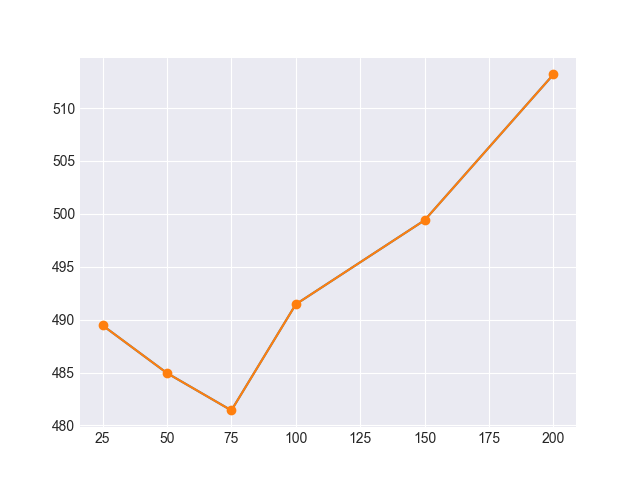
\includegraphics[width=\textwidth]{figures/lda-perplexity.png}
    \caption{The perplexity scores for the different LDA models}
    \label{fig:lda-perplexity}
\end{figure}

\begin{figure}[h!]
    \centering
    \thirdsubfigimg{invalid_reports_most_likely_topics_histogram}{The distribution of the topics with the highest probability for the invalid reports in the training set.}
    \thirdsubfigimg{valid_reports_most_likely_topics_histogram}{The distribution of the topics with the highest probability for the valid reports in the training set.}
    \caption{Distribution over the most likely topics for the valid and invalid reports. Note that only topics that occurred at least once are shown in the histogram.}
    \label{fig:most-likely-topics}
\end{figure}

The next step was identifying the topics that were assigned to the invalid reports.
First, topic 1 and 17 were identified as interesting based on the word distribution they represented.
The most common terms for these two topics can be seen in Figure~\ref{fig:topic-wordclouds}.
To verify this, the labeled data was analyzed.
The distribution of the topics with the highest likelihood for the invalid reports in the training set can be seen in Figure~\ref{fig:invalid-reports-most-likely-topics}.
A couple of topics, 1 and 17 clearly stands out as the ones that most invalid reports gets assigned.
Specifically, topic 1 had a count of 131 reports from the invalid reports in the training set, and topic 17 had 358.
Some invalid reports have topics 0, 3, 9, 16, 47, 53, 58, 61, 62 as the most likely topic.
53 is the third most common, with a count of 3.

The corresponding plot for the valid reports can be seen in Figure~\ref{fig:valid-reports-most-likely-topics}.
There is a lot more variety among the most likely topics here.
Topics 1 and 17 occurs very infrequently.
Topic 1 occurs 0 times, while topic 17 occurs 2 times.
The third most common topic from the invalid reports, 53, occurs 28 times.
The ones having topic 17 had 4 and 8 prominent topics assigned to them.

Each topic that was assigned to a report with a probability above 10\% was considered to be a prominent topic.
The number of prominent topics for the invalid reports can be seen in Figure~\ref{fig:invalid-reports-prominent-topic-count}.
1, 2 and 3 number of prominent topics are the most common.
And there are barely any reports having more than 6.
The corresponding plot for the valid reports can be seen in Figure~\ref{fig:valid-reports-prominent-topic-count}.
In the case of valid reports, 6 is the most common number of prominent topics. 
The topics are a lot more spread out than in the case of the invalid reports.

\begin{figure}[h!]
    \centering
    \thirdsubfigimg{invalid_reports_prominent_topics_count_histogram}{The distribution of the number of prominent topics assigned to the invalid reports in the training set.}
    \thirdsubfigimg{valid_reports_prominent_topics_count_histogram}{The distribution of the number of prominent topics assigned to the valid reports in the training set.}
    \caption{The distribution of the number of prominent topics for the two categories.}
    \label{fig:prominent-topic-dist}
\end{figure}

Another idea was to evaluate whether or not 17 and 1 was among the most probable topics for the reports.
A simple evaluation of this on the set of valid reports showed that it was not a good approach.
For example, seeing if 17 or 1 had more than 10\% probability returned 48 and 45 valid reports, respectively.
Checking if both were above the threshold returned 11 reports.
This threshold was tested with 1\% increments from 5\% to 20\% without giving any good results.

Based on these findings, reports were determined to be invalid or not by the following criterion:
\begin{itemize}
    \item Having either topic 1 or 17 as its most probable topic.
    \item Not having more than 6 prominent topics assigned to it.
\end{itemize}

The evaluation on the validation set can be seen in Table~\ref{tab:exp1-eval}.
In the figure you can also see the results of the logistic regression classifier, which was fitted with the topic vectors as features and the invalid/valid labels as targets.

\begin{table}[h!]
    \centering
    \begin{tabular}{|c|cc|}
        \hline
        & \textbf{Manual Identification} & \textbf{Logistic Regression} \\
        \hline
        \textbf{Precision} & 97.2\% & 98.7\% \\
        \textbf{Recall} & 100\% & 100\% \\
        \textbf{$F_1$-measure} & 98.6\% & 99.4\%\\
        \textbf{Accuracy} & 97.9\% & 99.1\%\\
        \hline
    \end{tabular}
    \caption{The results of the classification of the invalid reports. The manual identification column represents the use of manual interpretation of the LDA topics to find the invalid reports.}
    \label{tab:exp1-eval}
\end{table}

\section{Alternatives to Labeling at Random}

The first thing that was done with regards to this experiment was to explore and try to find a relationship between the initial set of labels and the inherit structure of the data.
This was done by visualizing the LDA model again.
In order to find any existing relationship between the topics and the labeled samples, the points were colored based on their assigned labels.
Unlabeled samples were hidden from the plot.
The resulting plot can be seen in Figure~\ref{fig:categories-lda-75}.
From this plot it is clear that there is a grouping of labels.
Certain labels are more likely to occur in documents assigned a specific topic.
For example, the purple points in the lower part of the graph represents the ``blödning'' label, the gray labels in the middle represents ``infarkt'' and the light blue ones that are mostly concentrated in the bottom right corner represents ``infektion''.
It is clear that these labels are not evenly spread out over all the topics, but neither are they confined enough to make a mapping between topics and labels, like they were in Section~\ref{sec:exp1-result}.

\begin{figure}[ht!]
    \centering
    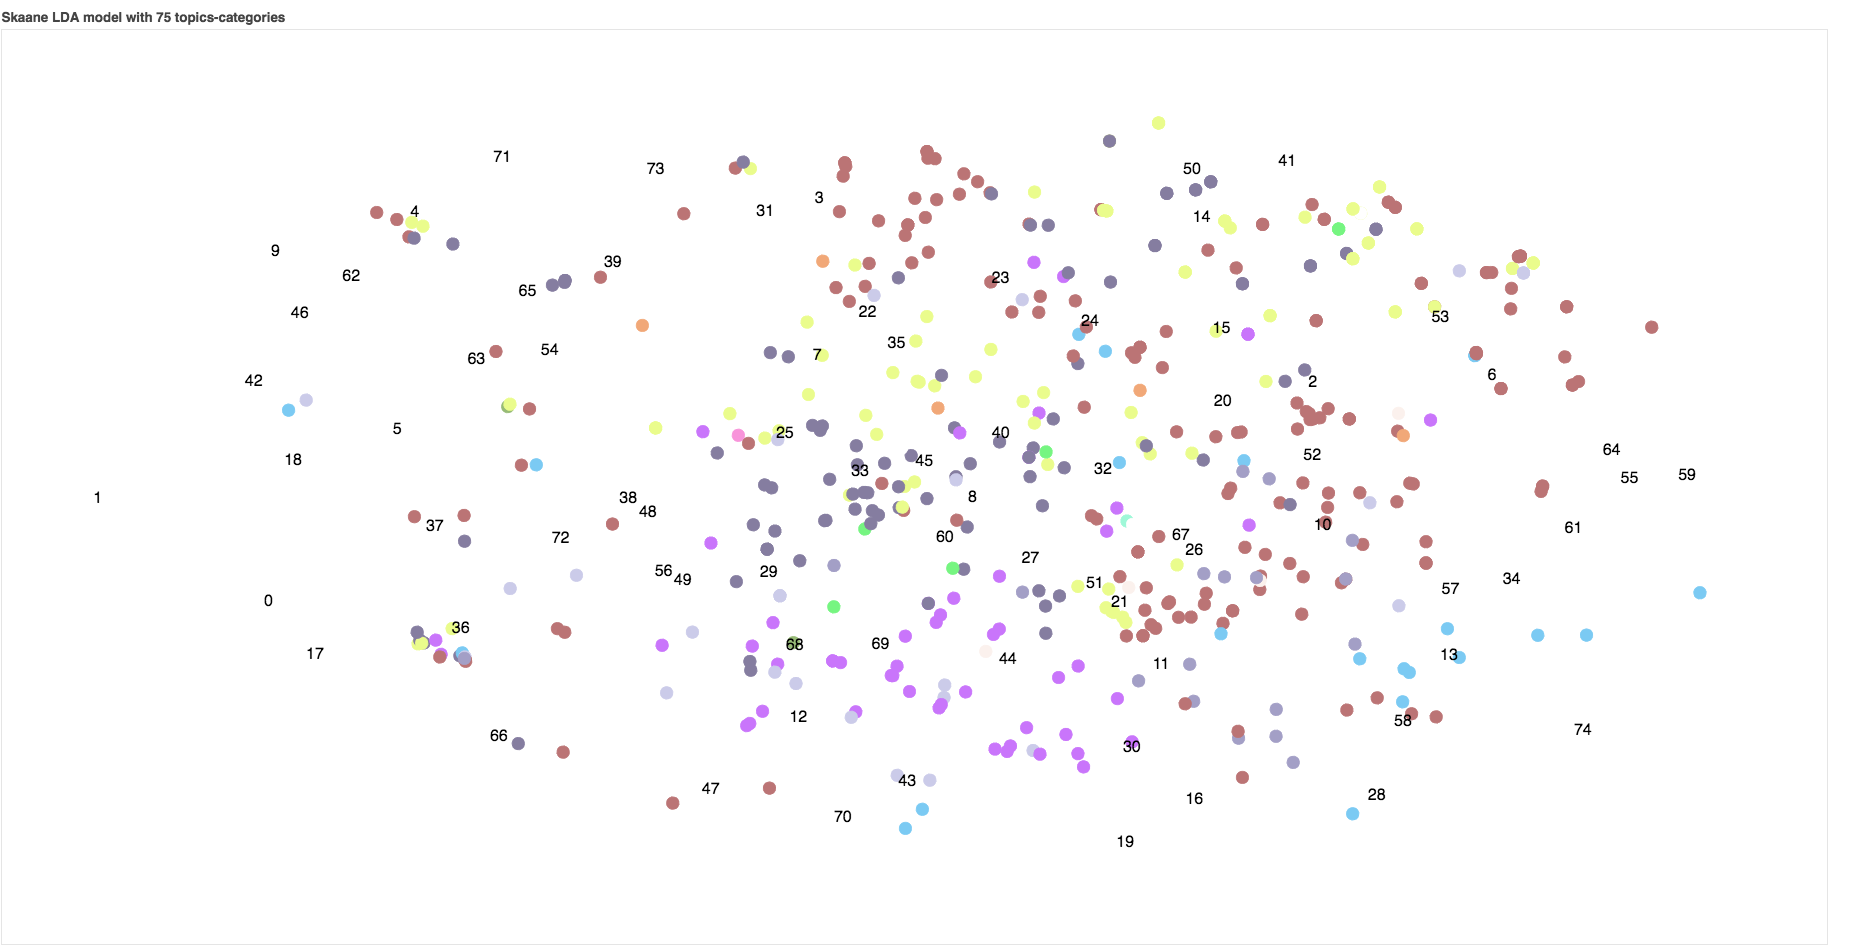
\includegraphics[width=\textwidth]{figures/categories-lda-75.png}
    \caption{The labeled data points plotted in 2D, and colored based on the first label of the report in alphabetical order.}
    \label{fig:categories-lda-75}
\end{figure}

In Figure~\ref{fig:category-label-distribution} the counts of most likely topics for the four most common categories are displayed.
These categories are ``infarkt'', ``kärlsjukdom'', ``normal'' and ``blödning''.
From the histograms it is clear that documents of a certain category are more likely to be assigned certain topics, at least in these cases.
Even though there exist a clear relationship, it is not exclusive enough to make any clear relation.
The number of topics assigned and reports labeled for these 4 topics can be seen in Table~\ref{tab:topic-categories}.

\begin{table}[ht!]
    \centering
    \begin{tabular}{|c|cc|}
        \hline
        \textbf{Label} & \textbf{No. reports} & \textbf{No. most likely topics} \\
        \hline
        Normal & 181 & 28\\
        Tumör & 29 & 15\\
        Infarkt & 105 & 27\\
        Blödning & 69 & 19\\
        Kärlsjukdom & 145 & 28\\
        Hydrocefalus & 10 & 5\\
        Demens & 14 & 9\\
        Trauma & 27 & 12\\
        Cysta & 9 & 7\\
        Missbildning & 3 & 3\\
        Inklämmning & 4 & 1\\
        Infektion & 29 & 15\\
        Syndrom & 2 & 2\\
        Metabol & 1 & 1\\
        \hline
    \end{tabular}
    \caption{The number of reports assigned a certain category, as well as the number of different topics assigned as the most likely one for reports with the given category.}
    \label{tab:topic-categories}
\end{table}

\begin{figure}[h!]
    \centering
    \thirdsubfigimg{infarkt}{The counts of most likely topics for the ``infarkt'' label.}
    \thirdsubfigimg{karlsjukdom}{The counts of most likely topics for the ``kärlsjukdom'' label.}
    \quad
    \thirdsubfigimg{normal}{The counts of most likely topics for the ``normal'' label.}
    \thirdsubfigimg{blodning}{The counts of most likely topics for the ``blödning'' label.}
    \caption{The counts of the most likely topics for the four most common categories.}
    \label{fig:category-label-distribution}
\end{figure}

In order to analyze these topics further, Figure~\ref{fig:topic-category-distribution} shows the different categories that has a certain topic assigned to it as the most likely one.
Taking into account the information from Table~\ref{tab:topic-categories}, i.e. that some categories are a lot more common than others in the labeled dataset, there is not a clear enough pattern to distinguish between different categories based on the topics.
This does not take the multi-label nature of the data into account.
If a report has multiple labels assigned to it, both of the labels are counted separately.

\begin{figure}[h!]
    \centering
    \thirdsubfigimg{categories-topic-13}{The counts categories where the most likely topic for the report was 13.}
    \thirdsubfigimg{categories-topic-16}{The counts categories where the most likely topic for the report was 16.}
    \quad
    \thirdsubfigimg{categories-topic-25}{The counts categories where the most likely topic for the report was 25.}
    \thirdsubfigimg{categories-topic-35}{The counts categories where the most likely topic for the report was 35.}
    \caption{The categories of the different reports that are assigned a certain topic as the most likely one.}
    \label{fig:topic-category-distribution}
\end{figure}

Based on the knowledge that there exists a pattern, the initial goal was to find some methods that could exploit this.
Some active learning approaches using different forms of clustering, such as Dasgupta et al\@'s approach using hierarchical clustering~\cite{dasgupta2008hierarchical}, would be good contenders.
However, the method described by Dasgupta et al\@. is made for the single-label case with no obvious way of extending the technique into multi-label.
The same applies to the density based technique suggested by Attenberg et al\@.~\cite{attenberg2013class}.

Most of the active learning research seems to be focused on binary, or maybe multi-class classification.
Thus the methods described in Section~\ref{sec:active-learning} where the ones decided on.
Methods that are fully reliant on a models certainty, such as Binary Version Space Minimization~\cite{brinker2006active} are used.
Furthermore, methods incorporating some information about the data in the form of label cardinality is included as well.
These techniques are MMC and Adaptive Active Learning~\cite{yang2009effective, li2013active}.
An attempt to take advantage of the structure of the data is done by selecting the initial samples from different clusters, as described in Section~\ref{sec:exp2-method}.

The plot for evaluating accuracy on the strategies with initial sample sizes of 25, 50 and 100 can be seen in Figure~\ref{fig:al-accuracy-25}, Figure~\ref{fig:al-accuracy-50}, and Figure~\ref{fig:al-accuracy-100} respectively.
Note that when retrieving the initial sample from the clusters, only samples with label cardinality 1 was retrieved after 10 tries.
MMC requires at least two different label cardinalities in the initial sample in order for the logistic regression model to work.
For that reason, MMC with cluster initialization was not evaluated.
In Table~\ref{tab:active-learning-accuracy-25} to Table~\ref{tab:active-learning-accuracy-100} it can be seen how many labels were required to reach a certain accuracy.

\includeaccuracyplot{25}
\includeaccuracyplot{50}
\includeaccuracyplot{100}

\begin{table}
    \centering
    \begin{tabular}{|cccccccc|}
        \hline
        \textbf{Strategy} & \textbf{Initial Sample} & \textbf{75 \%} & \textbf{80 \%} & \textbf{85 \%} & \textbf{87 \%} & \textbf{89 \%} & \textbf{89 \%}\\
        \hline
        BinMin & Random & 475 & 650 & 1100 & 1450 & 1675 & 2425\\
        BinMin & Cluster & 425 & 650 & 1100 & 1575 & 1700 & 2425\\
        MMC & Random & 600 & 775 & 1050 & 1250 & 1575 & N/A\\
        MMC & Cluster & N/A & N/A & N/A & N/A & N/A & N/A\\
        Adaptive & Random & 400 & 575 & 975 & 2425 & N/A & N/A\\
        Adaptive & Cluster & 375 & 550 & 1025 & 2300 & N/A & N/A\\
        Random & Random & 550 & 900 & 1700 & N/A & N/A & N/A\\
        \hline
    \end{tabular}
    \caption{The number of labeled reports in total that the strategies required to achieve the different accuracy values, with initial sample size 25.}
    \label{tab:active-learning-accuracy-25}
\end{table}

\begin{table}
    \centering
    \begin{tabular}{|cccccccc|}
        \hline
        \textbf{Strategy} & \textbf{Initial Sample} & \textbf{75 \%} & \textbf{80 \%} & \textbf{85 \%} & \textbf{87 \%} & \textbf{89 \%} & \textbf{89 \%}\\
        \hline
        BinMin & Random & 450 & 625 & 1075 & 1550 & 1750 & N/A\\
        BinMin & Cluster & 450 & 675 & 1125 & 1600 & 1725 & 2450\\
        MMC & Random & 625 & 775 & 1100 & 1325 & 1675 & N/A\\
        MMC & Cluster & N/A & N/A & N/A & N/A & N/A & N/A\\
        Adaptive & Random & 375 & 575 & 925 & N/A & N/A & N/A\\
        Adaptive & Cluster & 425 & 575 & 1075 & N/A & N/A & N/A\\
        Random & Random & 550 & 775 & 1575 & N/A & N/A & N/A\\
        \hline
    \end{tabular}
    \caption{The number of labeled reports in total that the strategies required to achieve the different accuracy values, with initial sample size 50.}
    \label{tab:active-learning-accuracy-50}
\end{table}

\begin{table}
    \centering
    \begin{tabular}{|cccccccc|}
        \hline
        \textbf{Strategy} & \textbf{Initial Sample} & \textbf{75 \%} & \textbf{80 \%} & \textbf{85 \%} & \textbf{87 \%} & \textbf{89 \%} & \textbf{89 \%}\\
        \hline
        BinMin & Random & 400 & 600 & 1125 & 1525 & 1775 & N/A\\
        BinMin & Cluster & 450 & 675 & 1125 & 1600 & 1725 & 2450\\
        MMC & Random & 600 & 750 & 1100 & 1325 & 1675 & N/A\\
        MMC & Cluster & N/A & N/A & N/A & N/A & N/A & N/A\\
        Adaptive & Random & 350 & 525 & 925 & 2450 & N/A & N/A\\
        Adaptive & Cluster & 450 & 600 & 1025 & N/A & N/A & N/A\\
        Random & Random & 475 & 775 & 1700 & N/A & N/A & N/A\\
        \hline
    \end{tabular}
    \caption{The number of labeled reports in total that the strategies required to achieve the different accuracy values, with initial sample size 100.}
    \label{tab:active-learning-accuracy-100}
\end{table}

The micro and macro $F_1$-score, recall and precision for the initial sample size of 25 can be seen in Figure~\ref{fig:result-25}.
The same evaluation for the initial sample size of 50 and 100 can be seen in Figure~\ref{fig:result-50} and Figure~\ref{fig:result-100}, respectively.

\includeevaluationplot{25}
\includeevaluationplot{50}
\includeevaluationplot{100}

\section{Evaluating the Label Balance}

The last part to evaluate is how the different Active Learning techniques effected the balance of the labels.
For the Reuters dataset, how the overall distribution of the labels is can be seen in Figure~\ref{fig:class-distribution-reuters}.
After random sampling, the distribution can be seen in Figure~\ref{fig:class-distribution-reuters-random}.
For comparison with the techniques it shows the labels both after 500 labels are added, and 2000.
The distribution after sampling with the original Binary Version Space Minimization can be seen in Figure~\ref{fig:class-distribution-reuters-binmin}, and with the initial samples taken from clusters in Figure~\ref{fig:class-distribution-reuters-binmin-clusters}.
For MMC the distribution can be seen in Figure~\ref{fig:class-distribution-reuters-mmc}.
The corresponding plots for Adaptive Active Learning can be seen in Figure~\ref{fig:class-distribution-reuters-adaptive} and Figure~\ref{fig:class-distribution-reuters-adaptive-clusters}.

\begin{figure}
    \centering
    \thirdsubfigimg{distribution-RandomSampling-25-500}{The class distribution from random sampling after 500 labels}
    \thirdsubfigimg{distribution-RandomSampling-25-2000}{The class distribution from random sampling after 2000 labels}
    \caption{The distribution of labels after random sampling}
    \label{fig:class-distribution-reuters-random}
\end{figure}

\begin{figure}
    \centering
    \thirdsubfigimg{distribution-BinaryMinimization-25-500}{The class distribution from Binary Version Space Minimization after 500 labels}
    \thirdsubfigimg{distribution-BinaryMinimization-25-2000}{The class distribution from Binary Version Space Minimization after 2000 labels}
    \caption{The distribution of labels after Binary Version Space Minimization}
    \label{fig:class-distribution-reuters-binmin}
\end{figure}


\begin{figure}
    \centering
    \thirdsubfigimg{distribution-ClusterBinaryMinimization-25-500}{The class distribution from Binary Version Space Minimization, with the initial sample from clusters, after 500 labels}
    \thirdsubfigimg{distribution-ClusterBinaryMinimization-25-2000}{The class distribution from Binary Version Space Minimization, with the initial sample from clusters, after 2000 labels}
    \caption{The distribution of labels after Binary Version Space Minimization with clustering}
    \label{fig:class-distribution-reuters-binmin-clusters}
\end{figure}

\begin{figure}
    \centering
    \thirdsubfigimg{distribution-MMC-25-500}{The class distribution from MMC after 500 labels}
    \thirdsubfigimg{distribution-MMC-25-2000}{The class distribution from MMC after 2000 labels}
    \caption{The distribution of labels after MMC}
    \label{fig:class-distribution-reuters-mmc}
\end{figure}

\begin{figure}
    \centering
    \thirdsubfigimg{distribution-AdaptiveLearner-25-500}{The class distribution from Adaptive Active Learning after 500 labels}
    \thirdsubfigimg{distribution-AdaptiveLearner-25-2000}{The class distribution from Adaptive Active Learning after 2000 labels}
    \caption{The distribution of labels after Adaptive Active Learning}
    \label{fig:class-distribution-reuters-adaptive}
\end{figure}

\begin{figure}
    \centering
    \thirdsubfigimg{distribution-ClusterAdaptiveLearner-25-500}{The class distribution from Adaptive Active Learning, with the initial sample from clusters, after 500 labels}
    \thirdsubfigimg{distribution-ClusterAdaptiveLearner-25-2000}{The class distribution from Adaptive Active Learning, with the initial sample from clusters, after 2000 labels}
    \caption{The distribution of labels after Adaptive Active Learning with clustering}
    \label{fig:class-distribution-reuters-adaptive-clusters}
\end{figure}

In Table~\ref{tab:distribution-result-500} the results of the evaluation after 500 new labels can be seen.
The corresponding table for the evaluation after 2000 new labels can be seen in Table~\ref{tab:distribution-result-2000}.

BinaryMinimization (24)
Biggest: 0.22031823745410037
Top 3  : 0.4981640146878825
Small  : 45.0


ClusterBinaryMinimization (24)
Biggest: 0.19753086419753085
Top 3  : 0.4901234567901235
Small  : 80.0


\begin{table}[h!]
    \centering
    \begin{tabular}{|ccccc|}
        \hline
        \textbf{Strategy} & \textbf{Initial Sample} & \textbf{Top Class} & \textbf{Top 3 Classes} & \textbf{Small/Big Ratio}\\
        \hline
        Random & Random &  34.9 \% & 65.5 \% & 32.0 \\
        BinMin & Random &  22.0 \% & 49.8 \% & 45.0 \\
        BinMin & Clusters & 19.8 \% & 49.0 \% & 80.0 \\
        Adaptive & Random & 14.8 \% & 38.5 \% & 5.4 \\
        Adaptive & Clusters & 14.5 \% & 38.2 \% & 6.65 \\
        MMC & Random & 13.1 \% & 35.2 \% & 8.2 \\
        \hline
    \end{tabular}
    \caption{The results after analyzing the label distribution after 500 new labels has been added.}
    \label{tab:distribution-result-500}
\end{table}

\begin{table}[h!]
    \centering
    \begin{tabular}{|ccccc|}
        \hline
        \textbf{Strategy} & \textbf{Initial Sample} & \textbf{Top Class} & \textbf{Top 3 Classes} & \textbf{Small/Big Ratio}\\
        \hline
        Random & Random & 36.65 \% & 64.6 \% & 29.4 \\
        BinMin & Random & 16.0 \% & 42.4 \% & 7.5 \\
        BinMin & Clusters & 15.7 \% & 41.5 \% & 7.3 \\
        Adaptive & Random & 36.4 \% & 56.2 \% & 43.4 \\
        Adaptive & Clusters & 34.5 \% & 54.8 \% & 41.0 \\
        MMC & Random & 16.7 \% & 41.2 \% & 9.3 \\
        \hline
    \end{tabular}
    \caption{The results after analyzing the label distribution after 2000 labels has been added.}
    \label{tab:distribution-result-2000}
\end{table}